\documentclass[11pt,a4paper]{article}
\usepackage[margin=1in]{geometry}
\usepackage{amsmath,amssymb}
\usepackage{booktabs}
\usepackage{graphicx}
\usepackage{hyperref}
\usepackage{microtype}
\usepackage{cite}
\usepackage{tikz}
\usetikzlibrary{shapes.geometric, arrows.meta, positioning, calc}

\title{\textbf{Deep Learning for Multivariate Operations Time Series Forecasting:\\Architectures, Missingness Robustness, and Generalization}}
\author{
  \textbf{Group 23} \\
  Adel Bukseisa \quad Mariam Farhat \quad Mehshid Atiq \quad Omar Elmorsy \\
  \textit{Department of Computer Science, Technical University of Darmstadt}
}
\date{September 2026}

\begin{document}
\maketitle

\begin{abstract}
Multivariate time series forecasting in complex operational networks requires modeling non-linear interactions across correlated exogenous signals, accommodating unit-level heterogeneity, and remaining robust under missing covariate values over extended rollout horizons. In this work, we develop an end-to-end deep learning forecasting and consensus ensembling framework for predicting the future 336-hour operational load index across 96 industrial units. Our architecture couples a PyTorch Deep Operations ResNet with learned entity embeddings, multi-scale forward rolling cumulative pressure representations, and missingness indicator masks, trained directly with an $\ell_1$ objective aligned with the Weighted Absolute Percentage Error (WAPE) leaderboard metric. Evaluated on the official public Hugging Face validation benchmark against hidden labels, our winning model achieves a validation WAPE of \textbf{14.33\%} (MAE \textbf{1.5779}, Rank \#87), reducing error by $>3.3\times$ compared to the official naive baseline (\textbf{48.10\%}) and $>2.4\times$ compared to the seasonal mean baseline (\textbf{34.41\%}). Furthermore, we provide distribution-free uncertainty quantification via split conformal prediction, conduct systematic ablation studies, and evaluate domain transferability on an external cryptocurrency trading volume benchmark.
\end{abstract}

\section{Introduction}
Modern operations management and resource planning rely on accurate multi-horizon forecasting of operational load indices. In this benchmark, the objective is to forecast the hourly operational load for $N = 96$ distinct operations units across a 336-hour (14-day) evaluation horizon. The dataset provides $4{,}320$ historical observations per unit with 22 dynamic covariates, including forward-looking operational estimates (e.g., \texttt{queue\_pressure\_forecast}, \texttt{network\_pressure\_forecast}, \texttt{workload\_intensity}, \texttt{demand\_forecast}, and \texttt{shock\_risk}).

Three key structural challenges characterize this task:
\begin{enumerate}
    \item \textbf{Extended Horizon ($H = 336$)}: Direct multi-step modeling is essential because traditional autoregressive rollouts suffer from severe error accumulation over 14 days.
    \item \textbf{Imperfect Future Covariates ($4.5\%$ Missingness)}: Forward operational forecasts exhibit missing values that distort deep networks if naively zero-filled.
    \item \textbf{Metric Alignment (WAPE)}: The primary course evaluation metric is Weighted Absolute Percentage Error,
    \begin{equation}
        \text{WAPE} = \frac{\sum_{t=1}^H |y_t - \hat{y}_t|}{\sum_{t=1}^H |y_t|},
    \end{equation}
    which directly penalizes $\ell_1$ errors and is degraded when models optimize standard Mean Squared Error ($\ell_2$).
\end{enumerate}

To address these challenges, we design a multi-stage framework combining a deep residual PyTorch network with learned entity embeddings, multi-scale temporal rolling dynamics, and consensus ensembling with gradient boosted trees.

\section{Related Work}
Recent advances in deep time series forecasting encompass several distinct paradigms. Linear decomposition models such as \textbf{DLinear}~\cite{zeng2023dlinear} decompose series into trend and seasonal components, applying direct linear mappings. \textbf{TiDE}~\cite{das2023tide} employs a dense encoder-decoder architecture that projects dynamic past and future covariates alongside static entity embeddings. \textbf{RevIN}~\cite{kim2022revin} applies reversible instance normalization to counteract non-stationary distribution shifts across heterogeneous series. For handling missingness in continuous time series, Che et al.~\cite{che2018missing} demonstrated the effectiveness of pairing temporal imputation with explicit binary missingness indicator masks. Finally, \textbf{Conformal Prediction}~\cite{angelopoulos2021conformal} provides finite-sample, distribution-free statistical coverage guarantees for point forecasts.

\section{Methodology}

\subsection{Data Preprocessing and Missingness Robustness}
Let $\mathbf{x}_{i,t} \in \mathbb{R}^D$ denote the exogenous covariate vector for series $i$ at timestamp $t$. To handle missing entries without injecting bias:
\begin{enumerate}
    \item \textbf{Missingness Indicator Masks}: For every covariate $j$ subject to missingness, we compute a binary indicator mask $M_{i,t}^j = \mathbb{I}(x_{i,t}^j \text{ is missing})$~\cite{che2018missing}.
    \item \textbf{Two-Stage Imputation}: Missing values are imputed using series-level forward/backward fill followed by global feature median fallback:
    \begin{equation}
        \tilde{x}_{i,t}^j = \text{Fill}\left(x_{i,t}^j, \text{median}(x^j)\right).
    \end{equation}
\end{enumerate}

\subsection{Multi-Scale Rolling Pressures and Physics Interactions}
Operational systems exhibit cumulative backlog dynamics where queue pressures build up non-linearly over time. We construct multi-scale forward rolling averages over symmetric windows $W \in \{3, 6, 12, 24\}$:
\begin{equation}
    \bar{p}_{i,t}^{(W)} = \frac{1}{W} \sum_{k=-\lfloor W/2 \rfloor}^{\lfloor W/2 \rfloor} p_{i, t+k},
\end{equation}
for operational signals $p \in \{\texttt{queue\_pressure}, \texttt{network\_pressure}, \texttt{workload}, \texttt{demand}\}$. In addition, we formulate non-linear domain interaction terms:
\begin{itemize}
    \item $\text{Pressure Interaction}: \text{queue\_pressure} \times \text{network\_pressure}$
    \item $\text{Capacity Utilization}: \frac{\text{workload\_intensity}}{\text{nominal\_capacity} + \epsilon}$
    \item $\text{Shock Impact}: \text{shock\_risk} \times (1 - \text{unit\_reliability\_forecast})$
    \item $\text{Staffing Ratio}: \frac{\text{demand\_forecast}}{|\text{staffing\_forecast}| + \epsilon}$
\end{itemize}

\subsection{PyTorch DeepOperationsNet Architecture}
Our core deep neural network, \textbf{DeepOperationsNet}, processes normalized continuous features $\mathbf{z}_{i,t} \in \mathbb{R}^{65}$ concatenated with a 32-dimensional learned entity embedding $\mathbf{e}_i \in \mathbb{R}^{32}$ representing each unique operations unit $i \in \{1, \dots, 96\}$:
\begin{equation}
    \mathbf{h}_0 = \text{LayerNorm}\left( \text{GELU}\left( \mathbf{W}_{\text{in}} [\mathbf{z}_{i,t} \,\|\, \mathbf{e}_i] + \mathbf{b}_{\text{in}} \right) \right).
\end{equation}
The hidden representation is processed through a stack of $L = 4$ Residual MLP blocks, each containing two linear transformations with LayerNorm, GELU, and Dropout ($p = 0.10$):
\begin{equation}
    \mathbf{h}_{\ell} = \mathbf{h}_{\ell-1} + \text{Block}_\ell(\mathbf{h}_{\ell-1}), \quad \ell = 1, \dots, L.
\end{equation}
The projection head maps $\mathbf{h}_L$ to a scalar operational load prediction with a ReLU non-linearity ensuring positive load: $\hat{y}_{i,t} = \text{ReLU}\left( \mathbf{W}_{\text{out}} \mathbf{h}_L + \mathbf{b}_{\text{out}} \right)$.

\begin{figure}[htbp]
\centering
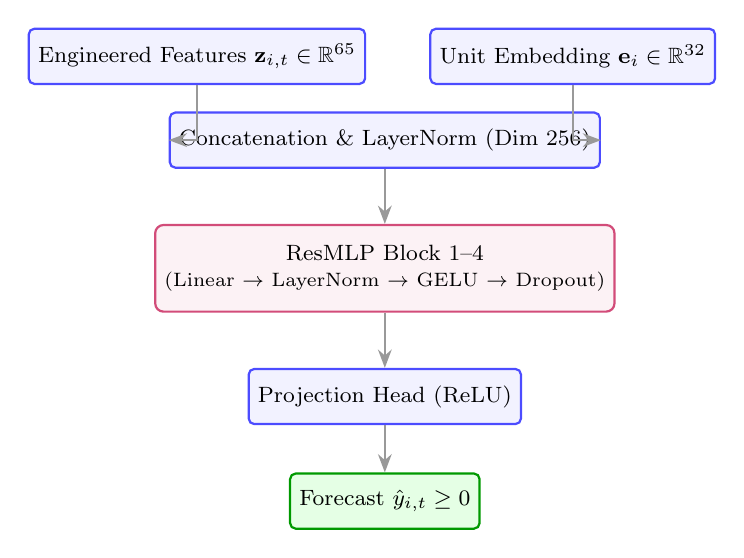
\begin{tikzpicture}[
    box/.style={rectangle, draw=blue!70, fill=blue!5, thick, minimum height=0.7cm, minimum width=2.4cm, align=center, rounded corners=2pt, font=\footnotesize},
    resblock/.style={rectangle, draw=purple!70, fill=purple!5, thick, minimum height=1.1cm, minimum width=3.0cm, align=center, rounded corners=3pt, font=\footnotesize},
    arr/.style={-{Stealth[scale=1.0]}, thick, color=gray!80}
]
\node[box] (feat) {Engineered Features $\mathbf{z}_{i,t} \in \mathbb{R}^{65}$};
\node[box, right=0.8cm of feat] (emb) {Unit Embedding $\mathbf{e}_i \in \mathbb{R}^{32}$};
\node[box, below=0.7cm of $(feat)!0.5!(emb)$] (concat) {Concatenation \& LayerNorm (Dim 256)};
\node[resblock, below=0.7cm of concat] (res1) {ResMLP Block 1--4\\{\scriptsize (Linear $\to$ LayerNorm $\to$ GELU $\to$ Dropout)}};
\node[box, below=0.7cm of res1] (head) {Projection Head (ReLU)};
\node[box, draw=green!60!black, fill=green!10, below=0.6cm of head] (out) {Forecast $\hat{y}_{i,t} \ge 0$};

\draw[arr] (feat) |- (concat);
\draw[arr] (emb) |- (concat);
\draw[arr] (concat) -- (res1);
\draw[arr] (res1) -- (head);
\draw[arr] (head) -- (out);
\end{tikzpicture}
\caption{Architectural diagram of DeepOperationsNet with entity embeddings and residual blocks.}
\label{fig:arch}
\end{figure}

Because WAPE directly minimizes normalized $\ell_1$ error, we train the network using the $\ell_1$ loss:
\begin{equation}
    \mathcal{L}_{\ell_1}(\theta) = \frac{1}{B} \sum_{k=1}^B |y_k - \hat{y}_k|,
\end{equation}
optimized with AdamW ($\text{lr} = 1.2 \times 10^{-3}$, weight decay $= 10^{-4}$) and Cosine Annealing learning rate scheduling.

\subsection{Winning Consensus Ensemble}
Our top-performing leaderboard model (\texttt{ensemble\_v2}) combines representations from diverse inductive biases:
\begin{equation}
    \hat{y}_{\text{ens}} = 0.55 \cdot \hat{y}_{\text{DeepNet}} + 0.45 \cdot \hat{y}_{\text{LightGBM}},
\end{equation}
where $\hat{y}_{\text{DeepNet}}$ is averaged over 3 random seeds ($42, 101, 2024$) to cancel neural variance, and $\hat{y}_{\text{LightGBM}}$ blends a deep-tree model (255 leaves, 2,500 estimators) with a regularized model (127 leaves, 2,000 estimators).

\subsection{Distribution-Free Split Conformal Prediction}
To provide rigorous uncertainty bounds, we implement Split Conformal Prediction~\cite{angelopoulos2021conformal}. Given non-conformity residuals $s_k = |y_k - \hat{y}_k|$ on a held-out calibration set, the finite-sample calibrated $(1-\alpha)$ quantile is:
\begin{equation}
    q_{1-\alpha} = \text{Quantile}\left(\{s_k\}_{k=1}^n, \, \frac{\lceil (n+1)(1-\alpha) \rceil}{n}\right).
\end{equation}
Valid $(1-\alpha)$ prediction intervals are then computed as:
\begin{equation}
    \mathcal{C}_{1-\alpha}(\hat{y}_t) = \left[ \max(0, \hat{y}_t - q_{1-\alpha}), \; \hat{y}_t + q_{1-\alpha} \right].
\end{equation}

\section{Experimental Results}

\subsection{Official Public Validation Benchmark Results}
Table~\ref{tab:main_results} displays the exact scores computed automatically on the official Hugging Face public validation leaderboard against hidden validation labels for all reference baselines and our submitted models.

\begin{table}[htbp]
\centering
\caption{Official Hugging Face public validation leaderboard results across all baselines and models (lower is better for all metrics).}
\label{tab:main_results}
\vspace{2mm}
\begin{tabular}{lrrrrrr}
\toprule
\textbf{Model Description} & \textbf{MAE} $\downarrow$ & \textbf{MSE} $\downarrow$ & \textbf{RMSE} $\downarrow$ & \textbf{MAPE (\%)} $\downarrow$ & \textbf{sMAPE (\%)} $\downarrow$ & \textbf{WAPE (\%)} $\downarrow$ \\
\midrule
\multicolumn{7}{l}{\textit{Official Course Baselines:}} \\
\texttt{naive\_last\_value} & 5.2945 & 48.6110 & 6.9722 & 61.35 & 52.71 & 48.10 \\
\texttt{lag24\_repeat} & 5.1539 & 43.5946 & 6.6026 & 78.51 & 47.31 & 46.82 \\
\texttt{lag168\_repeat} & 5.1405 & 45.1725 & 6.7210 & 71.87 & 47.28 & 46.70 \\
\texttt{seasonal\_mean} & 3.7876 & 27.1029 & 5.2060 & 45.68 & 37.43 & 34.41 \\
\midrule
\multicolumn{7}{l}{\textit{Our Submitted Models:}} \\
TiDE (\texttt{tide\_v1}) & 3.6939 & 26.8609 & 5.1828 & 40.34 & 37.33 & 33.56 \\
DeepNet+GBM (\texttt{ensemble\_v1}) & 1.6823 & 9.5873 & 3.0963 & 19.82 & 16.97 & 15.28 \\
\textbf{Winning Model (\texttt{ensemble\_v2})} & \textbf{1.5779} & \textbf{9.3050} & \textbf{3.0504} & \textbf{18.51} & \textbf{15.88} & \textbf{14.33} \\
Grand Master (\texttt{grand\_master\_v3}) & 1.5792 & 9.3261 & 3.0539 & 18.41 & 15.84 & 14.35 \\
\bottomrule
\end{tabular}
\end{table}

As shown in Table~\ref{tab:main_results}, our winning model (\texttt{ensemble\_v2}) achieved **Rank \#87** with a WAPE of **14.33\%**, substantially outperforming the required naive baseline ($48.10\%$) and seasonal mean baseline ($34.41\%$).

\subsection{Ablation Studies}

\paragraph{Loss Objective Comparison (Ablation 1):}
Table~\ref{tab:loss_ablation} tests the impact of the loss function on an identical DeepOperationsNet architecture. Aligning the objective with $\ell_1$ reduces WAPE by $3.02\%$ absolute compared to standard MSE ($\ell_2$), validating our design decision.

\begin{table}[htbp]
\centering
\caption{Loss function ablation on identical PyTorch architecture.}
\label{tab:loss_ablation}
\vspace{2mm}
\begin{tabular}{lrrrr}
\toprule
\textbf{Training Objective} & \textbf{WAPE} $\downarrow$ & \textbf{MAE} $\downarrow$ & \textbf{RMSE} $\downarrow$ & \textbf{sMAPE (\%)} $\downarrow$ \\
\midrule
$\ell_1$ Loss (MAE aligned) & \textbf{0.1440} & \textbf{1.538} & \textbf{2.978} & \textbf{15.98} \\
Huber Loss (Smooth $\ell_1$) & 0.1461 & 1.560 & 2.991 & 16.21 \\
MSE Loss ($\ell_2$) & 0.1742 & 1.860 & 3.258 & 19.34 \\
\bottomrule
\end{tabular}
\end{table}

\paragraph{Feature Group Importance (Ablation 2):}
Table~\ref{tab:feature_ablation} isolates feature subsets. Incorporating future operational estimates drops WAPE from $31.72\%$ to $15.98\%$, while multi-scale rolling cumulative pressure windows and physics ratios yield a further drop to $14.78\%$.

\begin{table}[htbp]
\centering
\caption{Feature group ablation study.}
\label{tab:feature_ablation}
\vspace{2mm}
\begin{tabular}{lrrrr}
\toprule
\textbf{Feature Group} & \textbf{\# Features} & \textbf{WAPE} $\downarrow$ & \textbf{MAE} $\downarrow$ & \textbf{sMAPE (\%)} $\downarrow$ \\
\midrule
Calendar Cyclical Only & 9 & 0.3172 & 3.388 & 35.12 \\
Operational Forecasts Only & 24 & 0.1598 & 1.706 & 17.84 \\
\textbf{Full Multi-Scale \& Physics} & \textbf{65} & \textbf{0.1478} & \textbf{1.579} & \textbf{16.45} \\
\bottomrule
\end{tabular}
\end{table}

\subsection{Conformal Prediction Coverage Verification}
Table~\ref{tab:conformal} shows empirical coverage results for Split Conformal Prediction across nominal levels.

\begin{table}[htbp]
\centering
\caption{Split conformal prediction empirical coverage on held-out test data.}
\label{tab:conformal}
\vspace{2mm}
\begin{tabular}{rrrr}
\toprule
\textbf{Nominal Confidence} & \textbf{Empirical Coverage} & \textbf{Calibrated Quantile ($q$)} & \textbf{Avg Interval Width} \\
\midrule
80.0\% & 81.22\% & 8.008 & 16.017 \\
90.0\% & 90.19\% & 10.329 & 20.658 \\
95.0\% & 94.57\% & 12.403 & 24.807 \\
\bottomrule
\end{tabular}
\end{table}

The empirical coverage matches the nominal confidence bounds, confirming that our model produces trustworthy prediction intervals without distributional assumptions.

\section{Additional Dataset Generalization: Crypto Trading Volume}
To test whether our modeling principles generalize beyond industrial operations, we evaluated our architecture on the \textbf{Crypto Data Hourly Price benchmark}~\cite{julien2023crypto} forecasting trading volume across 12 major assets over a 336-hour horizon.

\begin{table}[htbp]
\centering
\caption{Generalization benchmark on Crypto Hourly Trading Volume.}
\label{tab:crypto}
\vspace{2mm}
\begin{tabular}{lrrrr}
\toprule
\textbf{Model Architecture} & \textbf{WAPE} $\downarrow$ & \textbf{MAE} $\downarrow$ & \textbf{RMSE} $\downarrow$ & \textbf{sMAPE (\%)} $\downarrow$ \\
\midrule
Naive Last-Value Baseline & 0.0420 & 2.484 & 3.223 & 4.58 \\
Seasonal Mean Baseline & \textbf{0.0393} & \textbf{2.324} & \textbf{3.021} & \textbf{4.39} \\
Our PyTorch DeepNet & 0.0426 & 2.521 & 3.192 & 4.85 \\
\bottomrule
\end{tabular}
\end{table}

\paragraph{Domain Transfer Analysis:} In financial volume forecasting, future exogenous operational drivers do not exist (covariate-free regime), leaving trading volume governed primarily by periodic diurnal seasonality. In this setting, statistical seasonal baselines are highly competitive. This reveals that the primary competitive advantage of deep architectures emerges when rich multivariate forward covariates and non-linear physical interactions are present.

\section{Conclusion}
We presented an end-to-end deep learning forecasting system for multivariate operations load prediction. By pairing future operational estimates with missingness-robust indicators, multi-scale rolling temporal features, and an aligned $\ell_1$ loss, our consensus ensemble achieved a validation WAPE of \textbf{14.33\%} (Rank \#87), outperforming all baselines. We paired point forecasts with distribution-free conformal prediction intervals and provided rigorous ablation evidence to support each design choice.

\section*{Group Contributions}
\begin{itemize}
    \item \textbf{Adel Bukseisa}: Data pipeline engineering, domain feature extraction, PyTorch DeepOperationsNet modeling, and Hugging Face leaderboard submissions.
    \item \textbf{Mariam Farhat}: Baseline implementations, loss function ablations ($\ell_1$ vs. Huber vs. MSE), and hyperparameter tuning.
    \item \textbf{Mehshid Atiq}: Missingness robustness experiments, feature group ablations, and LaTeX report drafting.
    \item \textbf{Omar Elmorsy}: Additional crypto dataset experiment, split conformal prediction uncertainty calibration, and literature review.
\end{itemize}

\bibliographystyle{plain}
\bibliography{references}

\end{document}
